\documentclass[12pt]{article}
\usepackage{amssymb,amsmath, endnotes,setspace,enumerate,ulem,color,xspace,lscape}
\usepackage[sort]{natbib}
\usepackage{multicol}
\usepackage{graphicx}
\usepackage{subfig}
\usepackage{tabularx}
\usepackage{array}
\usepackage{float}
\usepackage{multirow}
\usepackage{booktabs}
\usepackage{caption}
\usepackage[bindingoffset=1.5cm, left=3cm, right=3cm, top=3cm, bottom=3cm]{geometry}
\allowdisplaybreaks[1]
\normalem
\newcommand{\textR}[1]{\textcolor{blue}{\texttt{#1}}}
\newcommand{\R}{\textR{R}}
\setlength{\columnsep}{.01cm}
\begin{document}
\sloppy


\title{Title of your project report}  

\author{
Sean Maloney\thanks{Department of Statistics.  Email: {\tt maloney4@wisc.edu}}  % 1st author
\and 
Sophia Margareta Carayannopoulos\thanks{Department of Statistics.  Email: {\tt  carayannopou@wisc.edu}}  % 2nd author
}

\maketitle

\begin{center}
\textbf{Abstract}
\end{center}

This is the abstract of your report ... 


\thispagestyle{empty}

\newpage

\pagenumbering{arabic} % add page numbers to your report

\section{Introduction}\label{intro}
\indent \indent Recently, cryptocurrencies have started to appear all over social and mainstream media. While the technology behind them is interesting what interests most people is the potential money. With bitcoin increasing over 10x in value during 2017 and the entire cryptocurrency ecosystem being measured in the hundreds of billions malicious actors might be trying to game the system through manipulated social media for their own financial gain.
\indent One of the main platforms used for cryptocurrency discussions is Reddit. The subreddit /r/CryptoCurrency/ has over 600k worldwide members and is specifically committed to the discussion and distribution of information about cryptocurrencies. 

Our goal to use the submissions and comments within /r/CryptoCurrency/ as metric of media hype to see if we could predict a cryptocurrency day to day performance .

\section{Gathering Data}\label{datagather}
\indent \indent Our data set from  /r/CryptoCurrency/ was collected from January 1, 2017 to December 31, 2017 and included all posts and comments. The dataset in total contains 5 million comments, 132k posts and 22k active users, active users being all unique accounts that posted or commented. We investigation will consider the top 10 coins (excluding bitcoin) by market cap on January 1, 2017 which from largest to smallest are as follows: Ethereum, Ripple, Litecoin, Monero, Ethereum Classic, Dash, MaidSafeCoin, Augar, Steem, NEM.

\indent Bitcoin is purposely excluded in our investigation as it is used as a baseline price unit. Each of the top 10 coin's prices will be considered in bitcoin value. Pricing in terms of bitcoin rather then USD is important as all of the coins we consider are traded directly to bitcoin rather then USD pairs.




\section{The Data Set}\label{dataset}

\indent \indent Our data set contained 26 predictor variables computed from the raw post and comment text. Each variable is computed over a single day. Each statistic for a coin has a corresponding control statistic for the day. This is important as the total number of posts and comments increased significantly throughout the year, see Figure 1.

\begin{figure}

\centering
  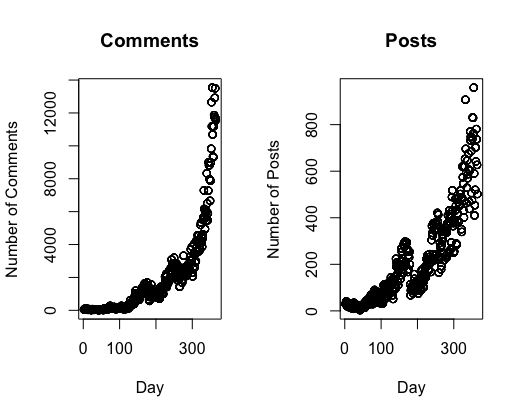
\includegraphics[width=\linewidth]{images/TotalCommentsPosts.png}
 \caption{Comment and Post Trends}
\label{label}

\end{figure}

The control prediction and coin prediction variables are listed and described (when unclear) below:

\subsection{Control Variables}

 \indent All statistics are computed for over a single day for all posts and comments.
\begin{enumerate}
\item Total Number Comments
\item Total Mean Comment Length

\indent Comment raw text length in characters

\item Total Comment Different Authors

\indent Total unique authors for both comments and posts based on username

\item Total Mean Comment Score Per Comment

\indent The mean comment score corresponds to the mean of the sum of upvotes and downvotes where upvotes and downvotes all have equal weight

\item Total Comment Number Fomo

\indent Number of times ?Fomo? or ?fear of missing out? appears as a literal in raw comment text

\item Total Comment Number Fud

\indent Number of times ?FUD? or ?fear, uncertainty and doubt? appears as a literal in raw comment text

\item Total Number Posts

\indent Total number of posts in /r/CryptoCurrency	

\item Total Post Mean Score

\indent The mean post score corresponds to the mean of the sum of upvotes and downvotes where upvotes and downvotes all have equal weight

\item Total Posts Mean Length

\indent Mean text length of all posts in characters

\item Total Posts Number Different Authors

\indent Number of unique authors over all posts
	
\item Total Posts Mean Number Of Comments

\indent Mean number of comments posts receive 

\item Total Posts Number Fomo

\indent Number of times ``Fomo'' or ``fear of missing out'' appears as a literal in raw posts text

\item Total Posts Number ``Fud''

\indent Number of times ``FUD'' or ?fear, uncertainty and doubt? appears as a literal in raw posts text 
\end{enumerate}

\subsection{Coin Specific Variables}


\indent \indent For the coin specific variables the post or comment was determined to be ``for'' the coin if they contained the coins name or the coins trading abbreviation in their raw text. All statistics are computed for each coin over a single day in the same fashion are the control variables. They are listed below and follow the same descriptions are the control variables above:
\begin{multicols}{2}
\begin{enumerate}
\item Total Number Coin Comments
\item Total Mean Coin Comment Length
\item Total Number Coin Comments Different Authors
\item Total Mean Coin Comment Score
\item Total Coin Comment Number Fomo
\item Total Coin Comment Number Fud
\item Total Coin Number Submissions
\item Total Coin Mean Submissions Score
\item Total Coin Mean Submissions Length
\item Total Coin Number Submissions Different Authors
\item Total Coin Mean Submissions Number Of Comments
\item Total Coin Submissions Number Fomo
\item Total Coin Submissions Number Fud
\end{enumerate}
\end{multicols}

\section{Preliminary Look}
\indent \indent Our first step was to look at the bitcoin prices of each coin over the year. We saw that there were three possibly distinct price groups in Figure 1. Upon further inspection, it seemed that that one distinct price group was: Augur, Steem, Ethereum, Ethereum Classic, which we refer to as Group 1, which can be seen in Figure 3a. They each have a very easy to follow distribution, unimodal, and bell shaped. It seemed that those in Group 1 had a peak between days 100 and 200. Upon further inspection it seemed that they also shared a peak around days 160 to 180. 

\indent The next distinct price group, Group 2, seemed to be: Dash, Litecoin, Monero, Maidsafe. These coins did not have an easy to follow curve like coins from Group 1. They seemed multimodal, but they also seemed to share a specific peak between 200 and 300 as seen in Figure 3b. They all shared a 20 day peak as well between.

\indent There is finally Group 3, though they were not as complicated to follow as the second group, their trend was not like Group 1 and deserved to be a separate and distinct group. It is possible that this group is bimodal but they share a peak between day 100-200. When we looked closer we saw that this peak was between 120-150, leading us to further believe that this is a distinct group, Figure 3c.

\indent We could not discern why these coins fell into distinct groups based on the merits of the coins. For example Ethereum and Steem are in the same group. Ethereum is still one of the top traded coins today. Steem is more of a niche coin and is not widely used, yet they fall into the same group. There may be a confounding variable that would be able to help more fully explain the similar trends. It is also possible that they are just random.

\begin{figure}

\centering
  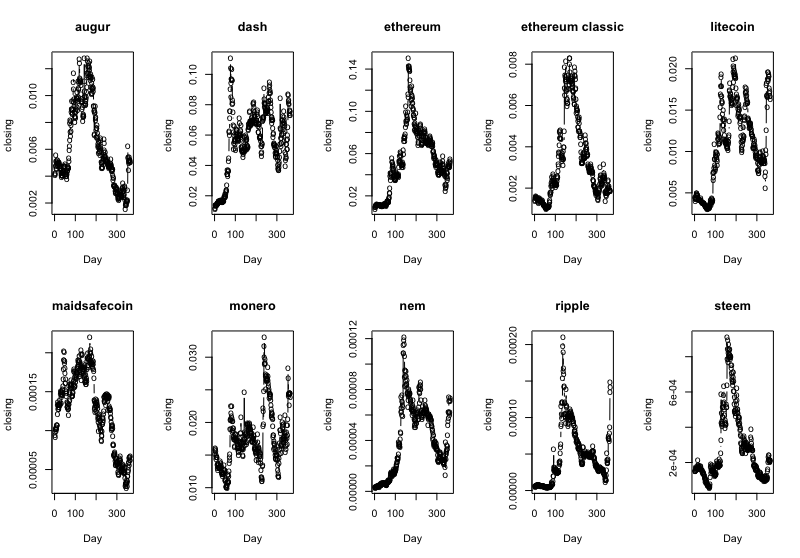
\includegraphics[width=\linewidth]{images/AllCoinTrends1.png}
 \caption{Trend of Each Coin}
\label{label}

\end{figure}

\begin{figure}[!tbp]
  \centering
  \subfloat[Group 1 Trends]{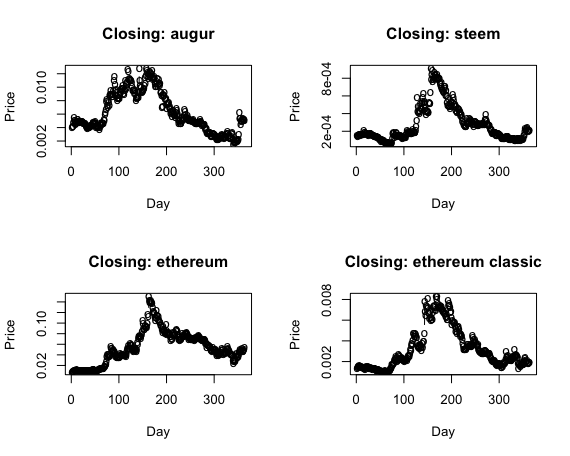
\includegraphics[width=0.4\textwidth]{images/Group1TrendsTotal.png}\label{fig:f1}}
  \hfill
  \subfloat[Group 2 Trends]{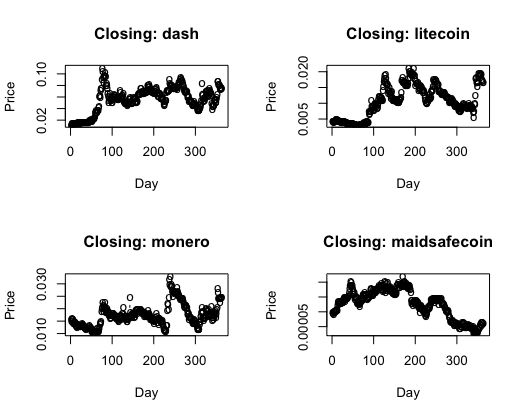
\includegraphics[width=0.4\textwidth]{images/Group2TrendsTotal.png}\label{fig:f2}}
    \hfill
  \subfloat[Group 3 Trends]{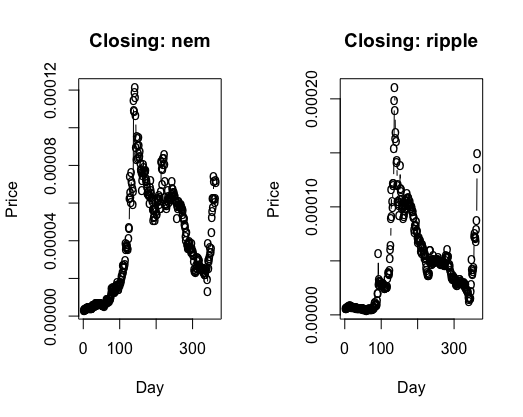
\includegraphics[width=0.4\textwidth]{images/Group3TrendsTotal.png}\label{fig:f3}}
  \caption{Trends By Groups}
\end{figure}

\begin{figure}

\centering
  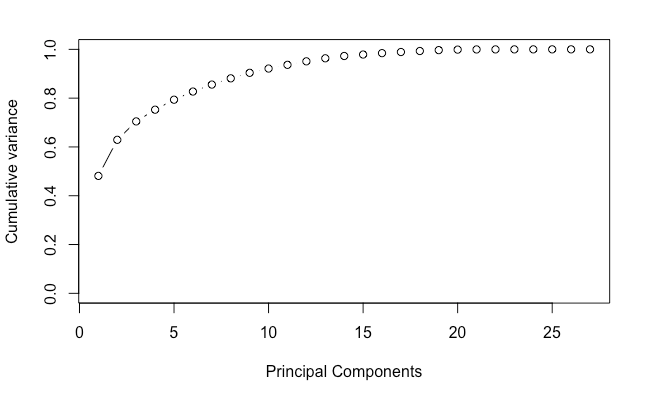
\includegraphics[width=\linewidth]{images/PCAFullModel.png}
 \caption{Measuring Variation Explained With Number Of Components}
\label{label}

\end{figure}


\section{Statistical Analysis}

\indent  \indent When we had set out to do this project we knew we wanted to do some kind of prediction of the value of the coin. We knew that with all of this information we would be unable to do a straightforward linear regression of any sort. Our first step was that we had to make all the variables more manageable. The next step was looking at the odds of whether or not the coin would rise in value. Finally we wanted to see how robust our model was. We felt that it would appropriate to build four models. One model would be using all the coins and the other three would be for each distinct group of coins. We wanted to see if separating them into groups would greatly improve the model, which would mean overfitting. Another thing we were looking for was to see if a certain group was making the model perform well while the other one or two were performing poorly.

\indent As mentioned above, we have a lot of variables that could be taken into account. They variables can also be correlated. It seemed that the most appropriate step would be to perform Principal Component Analysis, PCA. This technique is used for data sets like ours where we need to take the variables into a lower dimension. There are certain assumptions that need to be met before performing PCA. We are assuming that the variables have a linear relationship since PCA will be unable to detect nonlinear subspaces. An issue with that is we are not sure this holds for all of our variables, but we will hold the assumption that they are. Another assumption that is made before performing PCA is that we have a large and representative sample. There is no reason to believe that our dataset is not representative, let alone comprehensive. Once we performed PCA on all the variables except Coin, Close, High, Low, Open, we saw that to explain 80\% of the variation we need 5 variables, Figure 4. On closer inspection of the components, we could not find any of the variables more significantly weighted than others. This is another drawback of PCA, when compacting the data into a lower dimension you lose some interpretation and understanding of the data.

\indent Our next step was to use those components to fit a logistic regression model. We thought it would be interesting to see if we would be able to predict the odds if a coin went up or not. This made our logistic linear regression model a binomial one. One of the assumptions that could possibly be problematic is that we assume that all the variables are independent. Though we used PCA to deal with collinearity, it does not take away that a comment might influence an up vote and so on and so forth. We are working on the assumption that everyone can think for themselves and is not influenced by one another. There is the assumption, once again, that we need a large data set: we have met this. Due to using the component in our logistic regression, we did not feel it was appropriate to formal equation. For those who would like to see the model with the components fitted, the R code is included in the appendix
\indent After fitting the full model and the group models, we wanted to create confidence intervals for how often we are correct when the price goes up, when the price goes down, type I error, type II error. We decided that nonparametric bootstrap would be appropriate since we do not know that distribution of the population we are sampling from. For the assumption of bias, we might have potentially run into an issue. This is because we are testing the model with the same data we used to fit the model. Another assumption that is made is that is that the data set is large enough: there is no reason to believe that the data set is not large enough. When we created our confidence intervals for the above parameters we found that in general out model did not perform very well and had high type II errors, Tables 2. It seemed that Group 1 is the only group that performs decently but even then, it would not be enough that it would be likely that someone could be exploiting reddit for gain. There is also negative values in our confidence intervals. As we know it is impossible to get a negative amount correct or incorrect, but this shows how much variance is in our model.

\section{Conclusion}
\indent\indent Overall, our models do not perform well. From the variables that we selected it does not seem that someone can predict the odds of the coin going up in value. From our confidence intervals, we saw that our model is extremely variate and is therefore not good for prediction. We also saw that our type II error is quite high for most of the models. Groups 2 and Groups 3 were poorly fitted while Group 1 performed significantly better. Group 1 is also what contributed to the full model performing better. The model for Group 1 is still neither accurate nor precise enough to be considered a model that could be or could have been used for exploitation.

\section{Next Steps}

\indent\indent One of the issues might be that we were considering the appropriate variables to measure media hype. Looking at the karma of users or the up votes of users to indicate whether the odds of the value of the coin will go up. Another thing we can inspect more closely in the future is the coins in Group 1. As mentioned above, we could not find a reason as to why these coins grouped together. If we were to look in their relationship with our independent variables we might be able to understand why that model performed better than the others. That could also help us figure out which variables might be causing coins to be grouped together. Finally, we might change the focus of the next analysis. Working off the idea that we should be looking for other variables, we could look to see which accounts might be purposefully used to influence the value of a coin.




\begin{table}
\centering
\begin{tabular}{ |p{3cm}|p{3cm}|  }
\hline
\multicolumn{2}{|c|}{Labels} \\
\hline
Correct: Went Up & Type I Error \\
\hline
Type II Error &  Correct: Did Not Go Up \\
\hline
\end{tabular}
\caption{Labels for Tables}
\end{table}


\begin{table}[H]
\begin{tabular}{ |p{3cm}|p{3cm}|  }
\hline
\multicolumn{2}{|c|}{Full Model} \\
\hline
0.047 & .042 \\
\hline
0.418 &  0.490 \\
\hline
\end{tabular}
\quad
\begin{tabular}{ |p{3cm}|p{3cm}|  }
\hline
\multicolumn{2}{|c|}{Group 1} \\
\hline
0.028 & 0.022 \\
\hline
0.412 &  0.535 \\
\hline
\end{tabular}
\quad
\begin{tabular}{ |p{3cm}|p{3cm}|  }
\hline
\multicolumn{2}{|c|}{Group 2} \\
\hline
0.102 & 0.095 \\
\hline
0.367 &  0.434 \\
\hline
\end{tabular}
\quad
\begin{tabular}{ |p{3cm}|p{3cm}|  }
\hline
\multicolumn{2}{|c|}{Group 3} \\
\hline
0.187 & 0.148 \\
\hline
0.151 &  0.184 \\
\hline

\end{tabular}
\caption{Estimates}
\end{table}


\begin{table}[H]
\begin{tabular}{ |p{3cm}|p{3cm}|  }
\hline
\multicolumn{2}{|c|}{Full Model} \\
\hline
(-0.050, 0.145) & (-.046, 0.132) \\
\hline
(.334, 0.503) &  (.386, 0.595) \\
\hline
\end{tabular}
\quad
\begin{tabular}{ |p{3cm}|p{3cm}|  }
\hline
\multicolumn{2}{|c|}{Group 1} \\
\hline
(-0.026,0.083) & (-0.021,0.066) \\
\hline
(0.370,0.455) &  (0.471, 0.599) \\
\hline
\end{tabular}
\quad
\begin{tabular}{ |p{3cm}|p{3cm}|  }
\hline
\multicolumn{2}{|c|}{Group 2} \\
\hline
(-0.060,0.266) & (-0.048,0.239) \\
\hline
(0.223,0.51) &  (0.268,0.600) \\
\hline
\end{tabular}
\quad
\begin{tabular}{ |p{3cm}|p{3cm}|  }
\hline
\multicolumn{2}{|c|}{Group 3} \\
\hline
(0.103,0.478) & (0.068, 0.365) \\
\hline
(0.065, 0.368) & (0.089, 0.459)\\
\hline

\end{tabular}
\caption{Estimates}
\end{table}

\newpage


%%%%%%%%%%%%%%%%%%%%%%%%%%%%%%%%%%%%%%%%%%%%%%%%%%%%%%%%%%%%%%%%%%%%%%
%%%%%%%%%%%%%% Reference
%%%%%%%%%%%%%%%%%%%%%%%%%%%%%%%%%%%%%%%%%%%%%%%%%%%%%%%%%%%%%%%%%%%%%%
\bibliographystyle{apalike}

\bibliography{referencelist}
Frisvad, Jens C. Principal Component Analysis. www2.imm.dtu.dk/courses/27411/doc/Lection03/PCA2013.pdf.
?Assumptions of Logistic Regression.? Statistics Solutions, www.statisticssolutions.com/assumptions-of-logistic regression/.

Brems, Matt. ?A One-Stop Shop for Principal Component Analysis ? Towards Data Science.? Towards Data Science, Towards Data Science, 17 Apr. 2017, towardsdatascience.com/a-one-stop-shop-for-principal-component-analysis-5582fb7e0a9c



\newpage

%%%%%%%%%%%%%%%%%%%%%%%%%%%%%%%%%%%%%%%%%%%%%%%%%%%%%%%%%%%%%%%%%%%%%%
%%%%%%%%%%%%%%  Appendix
%%%%%%%%%%%%%%%%%%%%%%%%%%%%%%%%%%%%%%%%%%%%%%%%%%%%%%%%%%%%%%%%%%%%%%
\appendix
\sloppy
\begin{center}
\sloppy

{\Large {\bf Appendix: \R\ code}}
\end{center}

% INSERT R CODE HERE, 10 point font
{\footnotesize 

\begin{verbatim} 

#importing Data and setting up
all_coin_data = read.csv("all_coin_data.csv")

TOP_COINS = c(c("eth", "ethereum"), c("xrp","ripple"),c("ltc", "litecoin"),
c("xmr", "monero"),c("etc", "ethereum classic"),
c("dash", "dash"),c("maid", "maidsafecoin"), c("rep", "augur"), 
c("steem", "steem"), c("xem", "nem"))



#Playing With Data

###All Levels:
coins = levels(all_coin_data$Coin)

###Closing worth each day for a year.

par(mfrow=c(2,5))
for (i in coins) {
  plot(y= all_coin_data$Close[which(as.character(all_coin_data$Coin) == i)], 
  	x = all_coin_data$Day.1[which(as.character(all_coin_data$Coin) == i)], 
	main = i, type = 'b', pch = 'o', xlab="Day", ylab="closing ")
  
}


##Function for graphing groups
Setting_Window<- function(x){
  if( x == 1){
    par(mfrow=c(1,1))
  } else if(x == 2){
    par(mfrow=c(1,2))
  } else if( x == 3){
    par(mfrow=c(1,3))
  }else{
    par(mfrow=c(ceiling(x/2),ceiling(x/2)))
  }
}

plot_dot_closing <- function(groups, range_values){
  Setting_Window(length(groups))
  
  for (i in groups) {
    plot(y = all_coin_data$Close[which(all_coin_data$Coin == i & all_coin_data$Day.1 
    	>= range_values[1] & all_coin_data$Day.1 < range_values[2])], 
         x = all_coin_data$Day.1[which(all_coin_data$Coin == i & all_coin_data$Day.1 >=
         range_values[1] & all_coin_data$Day.1 < range_values[2])], 
         main = paste("Closing:", i), 
         type = 'b', pch = 'o', xlab= "Day", ylab = "Price")
  }
}

plot_dot_Total_Coin_Number_Comments <- function(groups, range_values){
  
  Setting_Window(length(groups))
  
  for (i in groups) {
    plot(y= all_coin_data$Total_Number_Coin_Comments[which(all_coin_data$Coin == i 
    & all_coin_data$Day.1 >= range_values[1] & all_coin_data$Day.1 
    < range_values[2])],   x = all_coin_data$Day.1[which(all_coin_data$Coin 
    == i & all_coin_data$Day.1 >= range_values[1] & all_coin_data$Day.1 
    < range_values[2])], main = paste("Total Number 
         Coin Comments", i), type = 'b', pch = 'o', xlab= "day", ylab = "Quantity")
  }
  
  
}

plot_dot_Total_Coin_Number_Submissions_FOMO <- function(groups, range_values){
  Setting_Window(length(groups))
  for (i in groups) {
    plot(y= all_coin_data$Total_Coin_Submissions_Num_Fomo[which(
    all_coin_data$Coin == i & all_coin_data$Day.1 >= range_values[1] 
    & all_coin_data$Day.1 < ange_values[2])], 
         x = all_coin_data$Day.1[which(all_coin_data$Coin == i & 
         all_coin_data$Day.1 >= range_values[1] & all_coin_data$Day.1 < 
         range_values[2])], main = paste("Total Number 
         Coin Submission FOMO", i), type = 'b', pch = 'o', xlab= "day", ylab = "Quantity")
  }
  
}

plot_dot_Total_Coin_Number_Submissions_FUD <- function(groups, range_values){
  Setting_Window(length(groups))
  
  for (i in groups) {
    plot(y= all_coin_data$Total_Coin_Submissions_Num_Fud[which(
    all_coin_data$Coin == i & all_coin_data$Day.1 >= range_values[1] & 
    all_coin_data$Day.1 <  range_values[2])], 
         x = all_coin_data$Day.1[which(all_coin_data$Coin == i & 
         all_coin_data$Day.1 >= range_values[1] & all_coin_data$Day.1
          < range_values[2])], main = paste("Total
          Number Coin Submissions FUD", i), type = 'b', pch = 'o', 
          xlab= "day", ylab = "Quantity")
  }
}

plot_dot_Total_Coin_Number_Comments_FOMO <- function(groups, range_values){
  Setting_Window(length(groups))
  for(i in groups){
    plot( y = all_coin_data$Total_Coin_Comment_Num_Fomo[which(
    all_coin_data$Coin   == i & all_coin_data$Day.1 >= range_values[1] 
    & all_coin_data$Day.1 < range_values[2])],
          x =  all_coin_data$Day.1[which(all_coin_data$Coin == i 
          & all_coin_data$Day.1 >= range_values[1] & all_coin_data$Day.1
           < range_values[2])], main = paste("Quanity 
          Comments FOMO", i), type = 'b', pch = 'o', xlab= "day", ylab = "Quantity")
  }
}

plot_dot_Total_Coin_Number_Comments_FUD <- function(groups, range_values){
  Setting_Window(length(groups))
  
  for(i in groups){
    plot( y = all_coin_data$Total_Coin_Comment_Num_Fomo
    [which(all_coin_data$Coin == i & all_coin_data$Day.1 >= 
    range_values[1] & all_coin_data$Day.1 < range_values[2])],
          x  = all_coin_data$Day.1[which(all_coin_data$Coin == i 
          & all_coin_data$Day.1 >= range_values[1] &
           all_coin_data$Day.1 < range_values[2])], main = paste("Quanity 
          Comments FUD", i), type = 'b', pch = 'o', xlab= "day", ylab = "Quantity")
  }
}

###Inspecting humps in first group
Group_1 <- c(coins[1], coins[10], coins[3], coins[4])
Group_1_orginal <- Group_1
plot_dot_closing(Group_1, c(100, 250))

#Seems that there is peaks in between 150 days and 200

plot_dot_closing(Group_1, c(150, 200))

#Looking at these graphs something is definitely going on between days 160 and 180

plot_dot_closing(Group_1, c(160, 175))

###Inspceting humps in the second group

Group_2 <- c(coins[2], coins[5], coins[7], coins[6])
Group_2_orginal = Group_2
plot_dot_closing(Group_2, c(200, 300))

#Definitely something between 220 and 280 for these coins. 
#interesting that this is at completely different time then group 1.
plot_dot_closing(Group_2, c(220,280))

#okay looking at these closer it seems like we should inspect between 230 and 250
plot_dot_closing(Group_2, c(230, 250))
#From here it seems that there is something going on with day 240ish, there seems to be a 
#change or something happening in particular

###Looking through group 3
Group_3 = c()
for( i in coins){
  if(!(i %in% Group_1) & !(i %in% Group_2)){
    Group_3 = c(Group_3, i)
  }
}
Group_3_Orginal <- Group_3
plot_dot_closing(Group_3, c(1, 365))
par(mfrow=c(2,1))
plot_dot_closing(Group_3, c(100, 200))
plot_dot_closing(Group_3, c(120, 180))
plot_dot_closing(Group_3, c(120, 150))

#So once again we have found a special hump. 


##SUMMARY AFTER LOOKING AT 3 GROUPS

  
###Looking At Comments in General.

mean(all_coin_data$Total_Number_Comments)
median(all_coin_data$Total_Number_Comments)
hist(all_coin_data$Total_Number_Comments )

par(mfrow=c(1,2))
plot(x = all_coin_data$Day.1, y = all_coin_data$Total_Number_Comments, xlab =  "Day",
 ylab = "Number of Comments")
plot(x = all_coin_data$Day.1, y = all_coin_data$Total_Number_Submissions, xlab =  "Day", 
ylab = "Number of Posts")

#100-200 Hump
par(mfrow=c(2,2))
plot(x = all_coin_data$Day.1[which(all_coin_data$Day.1 >= 100 & all_coin_data$Day.1 < 200)], 
y = all_coin_data$Total_Number_Comments[which(all_coin_data$Day.1
 >= 100 & all_coin_data$Day.1 < 200)], ylab= "comments", xlab = "day")

plot(x = all_coin_data$Day.1[which(all_coin_data$Day.1 >= 140 & 
all_coin_data$Day.1 < 200)], y = all_coin_data$Total_Number_Comments[
which(all_coin_data$Day.1 >= 140 & all_coin_data$Day.1 < 200)], 
ylab= "comments", xlab = "day")

plot(x = all_coin_data$Day.1[which(all_coin_data$Day.1 >= 160 & 
all_coin_data$Day.1 < 200)], y = all_coin_data$Total_Number_Comments[
which(all_coin_data$Day.1 >= 160 & all_coin_data$Day.1 < 200)], 
ylab= "comments", xlab = "day")

plot(x = all_coin_data$Day.1[which(all_coin_data$Day.1 >= 
160 & all_coin_data$Day.1 < 180)], y = all_coin_data$Total_Number_Comments[
which(all_coin_data$Day.1 >= 160 
& all_coin_data$Day.1 < 180)], ylab= "comments", xlab = "day")

#What type of comments
par(mfrow=c(2,1))
plot(all_coin_data$Day.1, all_coin_data$Total_Number_Comments, 
ylab= "comments", xlab = "day", main =  "Total Number Comments")
plot(all_coin_data$Day.1[which(all_coin_data$Day.1 >= 160 
& all_coin_data$Day.1 < 180)], all_coin_data$Total_Number_Comments
[which(all_coin_data$Day.1 >= 160
 & all_coin_data$Day.1 < 180)], ylab= "comments", xlab = "day", main =  
 "Total Number Comments 160-180")
plot_dot_Total_Coin_Number_Comments(Group_1, c(100,200))

#Oh you can totoally see that the comments for that time in all those coins. 
#So maybe # comments means something
#Let's start looking at comments more specifically.
plot(x = all_coin_data$Day.1, y=all_coin_data$Total_Coin_Comment_Num_Fomo, 
ylab= "Day", xlab="Quantity", main= "FOMO comments all coins")
cat("So Fomo looks like is increasing exponetially. ")

plot_dot_Total_Coin_Number_Comments(Group_1, c(1,365))
plot_dot_Total_Coin_Number_Comments_FOMO(Group_1, c(1,365))
plot_dot_Total_Coin_Number_Comments_FUD(Group_1, c(1,365))

plot_dot_Total_Coin_Number_Comments_FOMO(Group_1, c(160,180))
plot_dot_Total_Coin_Number_Comments_FUD(Group_1, c(160, 180))

plot_dot_Total_Coin_Number_Comments_FOMO(Group_1, c(140, 200))
plot_dot_Total_Coin_Number_Comments_FUD(Group_1, c(140, 200))

all_coin_data[which(all_coin_data$Day.1 < 180 & all_coin_data$Day.1 > 150 
& all_coin_data$Coin == "steem" & all_coin_data$Total_Coin_Comment_Num_Fomo == 1),"Day.1"]

all_coin_data[which(all_coin_data$Day.1 < 180 & all_coin_data$Day.1 > 150 
& all_coin_data$Coin == "steem" & all_coin_data$Total_Coin_Comment_Num_Fud == 1),"Day.1"]

#We see the humps of # comments also peaks at the same time their price peaks. 
#Possible peaks at the 160-180 mark

#Looking at Submissions in general and specifics

plot_dot_Total_Coin_Number_Submissions_FOMO(Group_1, c(1,365))
plot_dot_Total_Coin_Number_Submissions_FUD(Group_1, c(1, 365))

plot_dot_Total_Coin_Number_Submissions_FOMO(Group_1, c(140, 200))
plot_dot_Total_Coin_Number_Submissions_FUD(Group_1, c(140, 200))

plot_dot_Total_Coin_Number_Submissions_FOMO(Group_1, c(160, 180))
plot_dot_Total_Coin_Number_Submissions_FUD(Group_1, c(160, 180))

mean(all_coin_data$Total_Coin_Number_Submissions[which(all_coin_data$Day.1 <= 200 
& all_coin_data$Day.1 >= 180 & all_coin_data$Coin == "steem" )])

#Definitely looking like those humps mean something. Fud Submissions seem to be 
#about the coin seem to be as it starts to fall.


#200-300 Hump
par(mfrow=c(2,2))
plot(x = all_coin_data$Day.1[which(all_coin_data$Day.1 >= 200 
& all_coin_data$Day.1 < 300)], y = 
all_coin_data$Total_Number_Comments[which(all_coin_data$Day.1 >= 200 
& all_coin_data$Day.1 < 300)], ylab= "comments", xlab = "day")

plot(x = all_coin_data$Day.1[which(all_coin_data$Day.1 >= 220 
& all_coin_data$Day.1 < 280)], 
y = all_coin_data$Total_Number_Comments[which(all_coin_data$Day.1 >= 220 
& all_coin_data$Day.1 < 280)], ylab= "comments", xlab = "day")

plot(x = all_coin_data$Day.1[which(all_coin_data$Day.1 >= 230 
& all_coin_data$Day.1 < 270)], 
y = all_coin_data$Total_Number_Comments[which(all_coin_data$Day.1 >= 230 
& all_coin_data$Day.1 < 270)], ylab= "comments", xlab = "day")

plot(x = all_coin_data$Day.1[which(all_coin_data$Day.1 >= 240 
& all_coin_data$Day.1 < 260)], 
y = all_coin_data$Total_Number_Comments[which(all_coin_data$Day.1 >= 240 
& all_coin_data$Day.1 < 260)], ylab= "comments", xlab = "day")


#After looking
\end{verbatim} }



\end{document}


